\documentclass[9pt]{exam}

\usepackage{verbatim, multicol, tabularx, graphicx, float, color}
\usepackage{amsmath,amsthm, amssymb, latexsym, listings, qtree}

\lstset{frame=tb,
  language=Java,
  aboveskip=1mm,
  belowskip=0mm,
  showstringspaces=false,
  columns=flexible,
  basicstyle={\ttfamily},
  numbers=none,
  frame=single,
  breaklines=true,
  breakatwhitespace=true
}

\textwidth = 6.5 in
\textheight = 9 in
\oddsidemargin = 0.0 in
\evensidemargin = 0.0 in
\topmargin = -0.25 in
\headheight = 0.0 in
\headsep = 0.0 in
\parskip = 0.0in
\parindent = 0.0in

\def\ojoin{\setbox0=\hbox{$\bowtie$}%
  \rule[-.02ex]{.25em}{.4pt}\llap{\rule[\ht0]{.25em}{.4pt}}}
\def\leftouterjoin{\mathbin{\ojoin\mkern-5.8mu\bowtie}}
\def\rightouterjoin{\mathbin{\bowtie\mkern-5.8mu\ojoin}}
\def\fullouterjoin{\mathbin{\ojoin\mkern-5.8mu\bowtie\mkern-5.8mu\ojoin}}

\def\a{& $\blacksquare\blacksquare\blacksquare$ & [ B ] & [ C ] & [ D ] \\}
\def\b{& [ A ] & $\blacksquare\blacksquare\blacksquare$ & [ C ] & [ D ] \\}
\def\c{& [ A ] & [ B ] & $\blacksquare\blacksquare\blacksquare$ & [ D ] \\}
\def\d{& [ A ] & [ B ] & [ C ] & $\blacksquare\blacksquare\blacksquare$ \\}


\title{CS 4400-R Exam 1}
\date{Practice}
\setcounter{page}{0}
\begin{document}

\maketitle
\thispagestyle{head}
%% \firstpageheader{}
%%               {\tiny Copyright \textcopyright\ 2016 All rights reserved. Duplication and/or usage for purposes of any kind without permission is strictly forbidden.}
%%               {}


\runningheader{}
              {\tiny Copyright \textcopyright\ 2016 All rights reserved. Duplication and/or usage for purposes of any kind without permission is strictly forbidden.}
              {}

%% \footer{Page \thepage\ of \numpages}
%%               {}
%%               {Points available: \pointsonpage{\thepage} -
%%                points lost: \makebox[.5in]{\hrulefill} =
%%                points earned:  \makebox[.5in]{\hrulefill}.
%%               Graded by: \makebox[.5in]{\hrulefill}}


%% \ifprintanswers
%% \begin{center}
%% {\LARGE ANSWER KEY}
%% \end{center}
%% \else

\vspace{0.1in}

Name (print clearly): \ifprintanswers \underline{  {\bf ANSWER KEY}  } \fi \hrulefill Section: (e.g., B1) \makebox[.5in]{\hrulefill}

\vspace{0.25in}
\hbox to \textwidth{Signature: \hrulefill}

\vspace{0.25in}
\hbox to \textwidth{GT account username (gtg, gth, msmith3, etc): \enspace\hrulefill}

\vfill

\begin{itemize}
\item Signing signifies that you agree to comply with the {\bf Academic Honor Code of Georgia Tech}.
\item Calculators and cell phones are NOT allowed.
\end{itemize}


% Points Table
%\begin{center}
%\addpoints
%\gradetable[v][pages]
%\end{center}

Completely fill in the box corresponding to your answer choice for each question.

\ifprintanswers
\begin{tabular}{lcccc}\\
  1. \d
  2. \a
  3. \d
  4. \b
  5. \d
  6. \b
  7. \b
  8. \a
  9. \d
  10. \c
  11. \d
  12. \b
  13. \a
  14. \a
  15. \b
  16. \a
  17. \d
  18. \c
  19. \b
  20. \a
  21. \c
  22. \a
  23. \c
  24. \a
  25. \b
\end{tabular}
\else
\begin{tabular}{lcccc}\\
  1. & [ A ] & [ B ] & [ C ] & [ D ] \\
  2. & [ A ] & [ B ] & [ C ] & [ D ] \\
  3. & [ A ] & [ B ] & [ C ] & [ D ] \\
  4. & [ A ] & [ B ] & [ C ] & [ D ] \\
  5. & [ A ] & [ B ] & [ C ] & [ D ] \\
  6. & [ A ] & [ B ] & [ C ] & [ D ] \\
  7. & [ A ] & [ B ] & [ C ] & [ D ] \\
  8. & [ A ] & [ B ] & [ C ] & [ D ] \\
  9. & [ A ] & [ B ] & [ C ] & [ D ] \\
  10. & [ A ] & [ B ] & [ C ] & [ D ] \\
  11. & [ A ] & [ B ] & [ C ] & [ D ] \\
  12. & [ A ] & [ B ] & [ C ] & [ D ] \\
  13. & [ A ] & [ B ] & [ C ] & [ D ] \\
  14. & [ A ] & [ B ] & [ C ] & [ D ] \\
  15. & [ A ] & [ B ] & [ C ] & [ D ] \\
  16. & [ A ] & [ B ] & [ C ] & [ D ] \\
  17. & [ A ] & [ B ] & [ C ] & [ D ] \\
  18. & [ A ] & [ B ] & [ C ] & [ D ] \\
  19. & [ A ] & [ B ] & [ C ] & [ D ] \\
  20. & [ A ] & [ B ] & [ C ] & [ D ] \\
  21. & [ A ] & [ B ] & [ C ] & [ D ] \\
  22. & [ A ] & [ B ] & [ C ] & [ D ] \\
  23. & [ A ] & [ B ] & [ C ] & [ D ] \\
  24. & [ A ] & [ B ] & [ C ] & [ D ] \\
  25. & [ A ] & [ B ] & [ C ] & [ D ] \\
\end{tabular}

\fi

\vspace{.5in}

Number missed: \makebox[.5in]{\hrulefill} Final Score: \makebox[.5in]{\hrulefill}

\newpage

%\normalsize

\pointsinmargin
\bracketedpoints

\marginpointname{}
%%%%%%%%%%%%%%%%%%%%%%%%%%%%%%%%%%%%%%%%%%%%%%%%%%%%%%%%%%%%%%%%%%%%%%%%%%%%

\begin{questions}


\question[4] Which of the following is/are example(s) of metadata?

\begin{choices}
\choice Types of data elements
\choice Structure of records
\choice Constraints
\correctchoice All of the above
\end{choices}

\question[4] What is the first step in database development?

\begin{choices}
\correctchoice Requirements analysis
\choice Conceptual design
\choice Logical design
\choice Physical design
\end{choices}

\question[4] Which of the following are advantages of the database approach?

\begin{choices}
\choice Storing metadata with the data
\choice Insulation between data and programs.
\choice Multiple views of the data for different users.
\correctchoice All of the above.
\end{choices}

\question[4] Which database technology is most pervasive and the focus of this course?

\begin{choices}
\choice Hierarchical databases
\correctchoice Relational databases
\choice Object-oriented databases
\choice Document-oriented databases
\end{choices}

\question[4] Abstraction is ...

\begin{choices}
\choice selective ignorance.
\choice suppression of details.
\choice for a particular application.
\correctchoice All of the above
\end{choices}

\question[4] Data independence is ...

\begin{choices}
\choice the ability to store data on independent disks.
\correctchoice isolation of changes at one schema level from levels above it.
\choice the freedom to change the data without consulting the DBA.
\choice All of the above
\end{choices}

\newpage

\question[4] The primary goal of the three-schema database architecture is

\begin{choices}
\choice data integrity.
\correctchoice data independence.
\choice data cohesion.
\choice data processing.
\end{choices}

\question[4] External schemas

\begin{choices}
\correctchoice are views tailored to particular users
\choice are specified with ER models
\choice specify the storage structure of the data
\choice None of the above
\end{choices}

\question[4] Conceptual models

\begin{choices}
\choice provide a high-level but concrete view of data understandable by end users and database developers.
\choice are developed after requirements analysis.
\choice may influence changes in requirements as developers iterate the design with users.
\correctchoice All of the above
\end{choices}

\question[4] Entity-relationship models contain

\begin{choices}
\choice entities, relationships and SQL code.
\choice entities, constraints and storage schemas.
\correctchoice entities, attributes and relationships.
\choice mappings bewtween levels of the three-schema architecture.
\end{choices}

\question[4] Structural constraints between entity types and relationships include

\begin{choices}
\choice participation constraints.
\choice cardinality ratios.
\choice data types.
\correctchoice A and B above.
\end{choices}

\question[4] A weak entity has a key.

\begin{choices}
\choice True
\correctchoice False
\end{choices}

\newpage

Refer to the following EER diagram for the remaining questions.

\begin{center}
  \hspace{-.5in}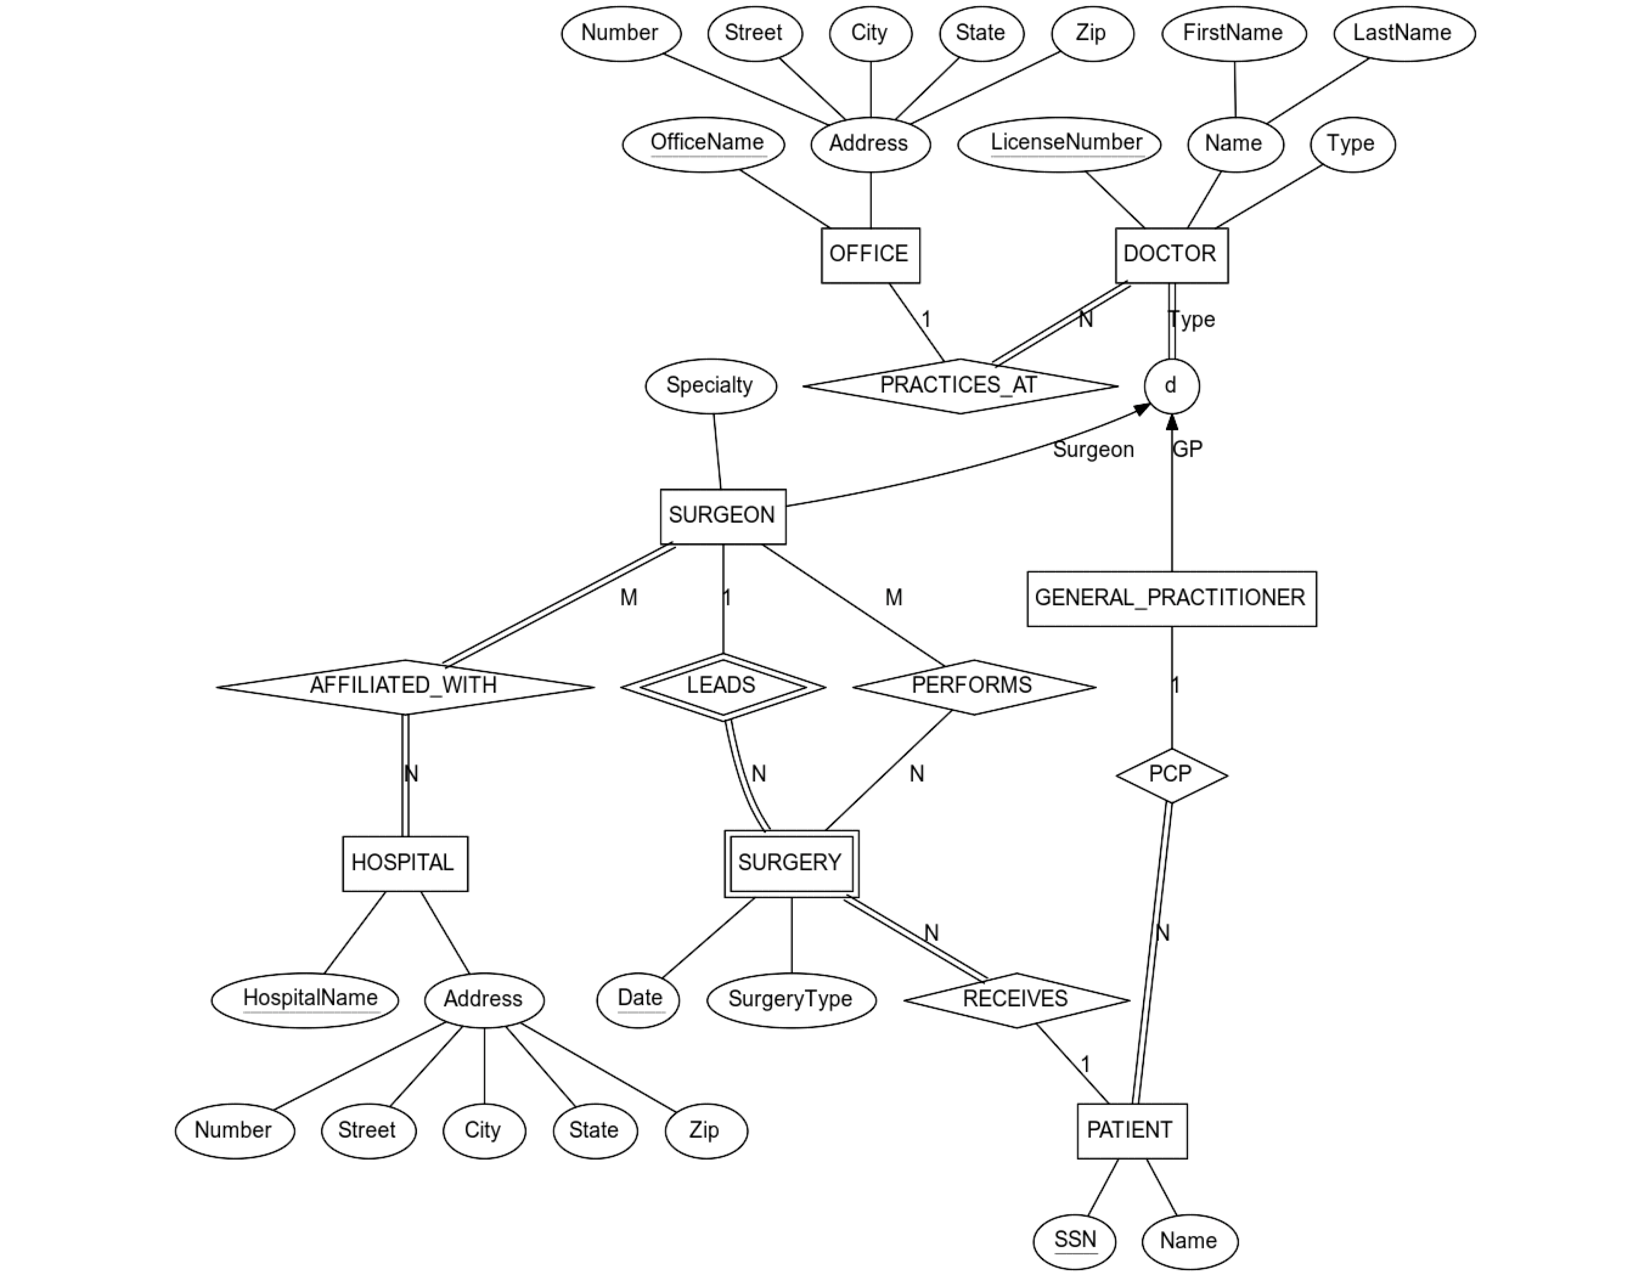
\includegraphics[width=7in]{doctors.pdf}
\end{center}

\newpage

\question[4] Can there be two OFFICE instances at the same Address?

\begin{choices}
\correctchoice Yes
\choice No
\end{choices}

\question[4] Can there be an OFFICE instance without any DOCTORs who PRACTICE\_AT that OFFICE?

\begin{choices}
\correctchoice Yes
\choice No
\end{choices}

\question[4] Can there be a DOCTOR instance that does not PRACTICE\_AT an OFFICE?

\begin{choices}
\choice Yes
\correctchoice No
\end{choices}

\question[4] How many OFFICEs may a DOCTOR PRACTICE\_AT?

\begin{choices}
\correctchoice 1
\choice 0 or more
\choice 1 or more
\end{choices}

\question[4] What is the full set of possible values for the Type attribute of DOCTOR?

\begin{choices}
  \choice \{'Surgeon', 'GP', 'ER', NULL\}
  \choice \{'Surgeon', 'GP', 'ER'\}
  \choice \{'Surgeon', 'GP', NULL\}
  \correctchoice \{'Surgeon', 'GP'\}
\end{choices}

\question[4] Making no assumptions about the number of instances of any other entity type, the number of SURGEON instances is \makebox[.25in]{\hrulefill} the number of DOCTOR instances.

\begin{choices}
\choice less than
\choice equal to
\correctchoice less than or equal to
\choice greater than
\end{choices}

\question[4] Can there be any DOCTOR instances that are not either SURGEON instances or GENERAL\_PRACTITIONER instances?

\begin{choices}
\choice Yes
\correctchoice No
\end{choices}

\question[4] Does the existence of a PATIENT instance imply the existence of an OFFICE instance?

\begin{choices}
\correctchoice Yes
\choice No
\end{choices}

\newpage

\question[4] If there are five SURGERY instances, how many DOCTOR instances are there?

\begin{choices}
\choice Five or more
\choice One or more
\correctchoice Two or more
\choice Cannot be determined from the information given
\end{choices}

\question[4] How many HOSPITALs must a SURGEON be AFFILIATED\_WITH?

\begin{choices}
\correctchoice One or more
\choice Zero or more
\choice More than 2
\end{choices}

\question[4] Which of the following is a valid key for a SURGERY instance?

\begin{choices}
\choice $<Date, SurgeryType>$
\choice $<SurgeryType, Specialty>$
\correctchoice $<LicenseNumber, Date>$
\choice $<Date, SurgeryType, SSN>$
\end{choices}

\question[4] Given this EER model, how may SURGERYs may a SURGEON LEAD on a given Date?

\begin{choices}
\correctchoice 1
\choice many
\choice none
\end{choices}

\question[4] Given this EER model, if we wanted the SurgeryType attribute for each SURGERY instance to have the same value as the Specialty attribute of the SURGEON who LEADs the surgery, we would enforce this correponsdence with a

\begin{choices}
  \choice data integrity constraint.
  \correctchoice semantic constraint/business rule.
  \choice participation constraint.
  \choice heuristic.
\end{choices}


\end{questions}

\end{document}
